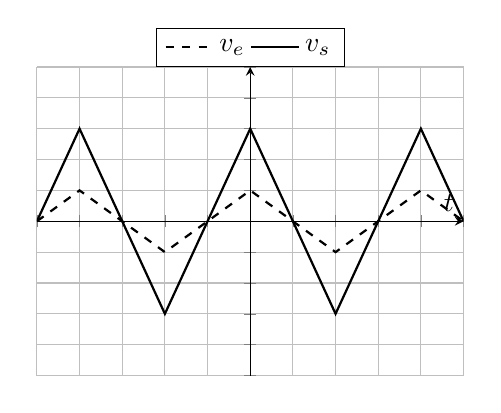
\begin{tikzpicture}
  \begin{axis}[
    xlabel = \(t\),
    ylabel = {} ,
    domain = -5:5,
    ymin = -5,
    ymax = 5,
    samples = 100,
    axis x line = center,
    axis y line = center,
    xtick = {-5, -4, ..., 5},
    ytick = {-5, -4, ..., 5},
    xticklabels = {},
    yticklabels = {},
    grid = both,
    width = 7cm,
    height = 5.5cm,
    legend columns=2, 
    legend style={at={(0.5,1.0)}, anchor=south}
    ]
    \addplot [thick, dashed] coordinates {(-5, 0) (-4, 1) (-2, -1)(0, 1)(2, -1)(4,1) (5,0)};
    \addlegendentry{\(v_e\)}
    \addplot [thick] coordinates {(-5, 0) (-4, 3) (-2, -3)(0, 3)(2, -3)(4,3) (5,0)};
    \addlegendentry{\(v_s\)}
  \end{axis}
\end{tikzpicture}